\documentclass{article}
\usepackage[utf8]{inputenc}
\usepackage{amsmath}
\usepackage{graphicx}
\usepackage{geometry}
\geometry{margin=2.5cm}
\usepackage{caption}
\usepackage{float}

\begin{document}

% Portada del examen
\begin{titlepage}
    \centering
    
\includegraphics[height=2.2cm]{fing.png}\hfill
    
\includegraphics[height=2.2cm]{uach.png}
    \\
    \vspace{1.5cm}
    {\Large \textbf{Universidad Autónoma de Chihuahua}}\\[0.2cm]
    {\large Facultad de Ingeniería}\\[0.5cm]
    {\Large \textbf{Métodos Numéricos}}\\[0.5cm]
    {\large Examen Parcial 2\_2}\\[1cm]

    \vspace{1.2cm}
    {\large Nombre: \underline{Francisco Javier Ponce Saenz}}\\[0.3cm]
    {\large Matrícula: \underline{a325000}}\\[0.3cm]
    {\large Semestre: \underline{3er Semestre}}\\[0.3cm]
    {\large Fecha: \underline{\hspace{4cm}}}\\
    \vfill
\end{titlepage}

\section*{Examen Parcial 2 Unidad 2}
\subsection*{Problema 1: Interpolación de Lagrange}
Se utiliza la interpolación de Lagrange con los puntos:
\begin{center}
\begin{tabular}{c c}
$x$ & $y$ \\
\hline
0 & -3 \\
1 & 0 \\
2 & 5 \\
3 & 12 \\
4 & 21 \\
5 & 32 \\
6 & 45 \\
7 & 50 \\
\end{tabular}
\end{center}

El polinomio interpolante de grado 7 es:
\[
P(x) = -\frac{1}{504}x^{7} + \frac{1}{24}x^{6} - \frac{25}{72}x^{5} + \frac{35}{24}x^{4} - \frac{29}{9}x^{3} + \frac{9}{2}x^{2} + \frac{4}{7}x - 3.
\]

Evaluando el polinomio en los puntos solicitados:
\begin{align*}
P(-3) &= 360,\\
P(-2) &= 77,\\
P(-1) &= 6.
\end{align*}

\begin{figure}[H]
    \centering
    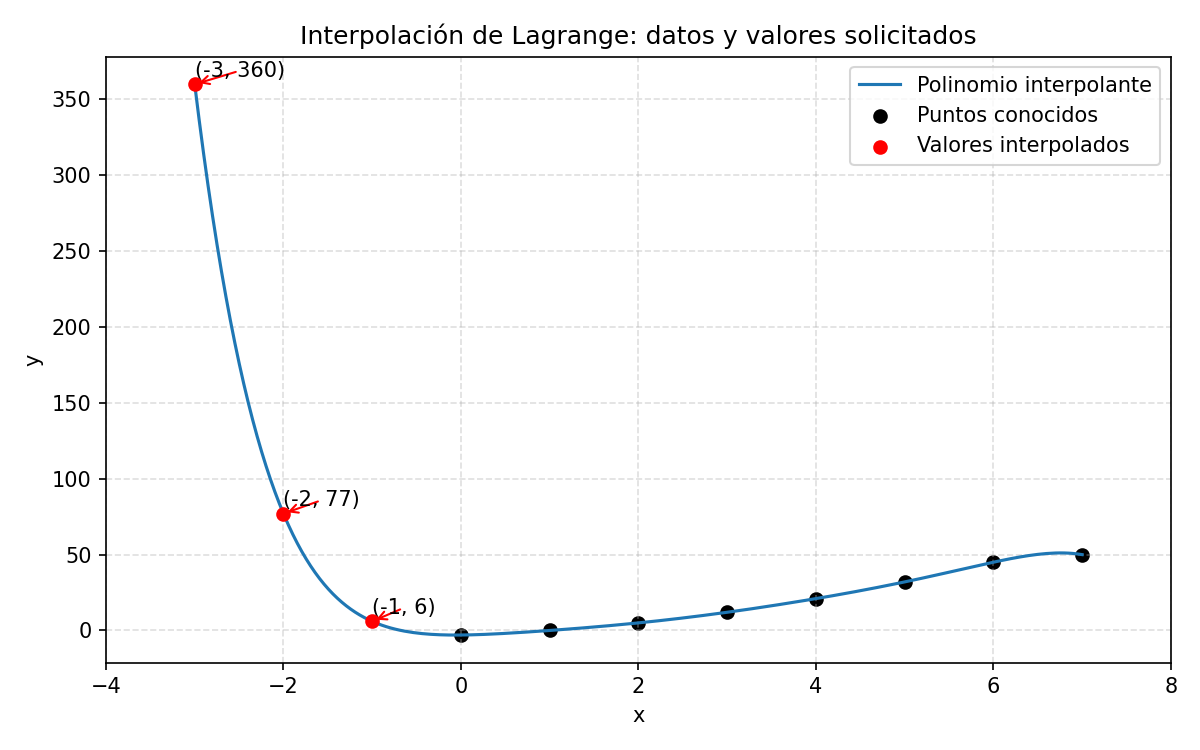
\includegraphics[width=0.75\textwidth]{lagrange_result.png}
    \caption{Captura de resultados de la interpolación de Lagrange.}
\end{figure}

\subsection*{Problema 2: Interpolación lineal}
\subsubsection*{a) Encontrar la abscisa con $y=-11$}
Los puntos son $(-5,-4)$ y $(3,-2)$.
La pendiente de la recta es:
\[
m = \frac{-2 - (-4)}{3 - (-5)} = \frac{2}{8} = \frac{1}{4}.
\]
La ecuación de la recta es:
\[
y + 4 = \frac{1}{4}(x + 5).
\]
Para $y=-11$ se obtiene:
\[
-11 + 4 = \frac{1}{4}(x + 5) \quad\Rightarrow\quad -7 = \frac{1}{4}(x + 5)
\]
\[
 x + 5 = -28 \quad\Rightarrow\quad x = -33.
\]

\begin{figure}[H]
    \centering
    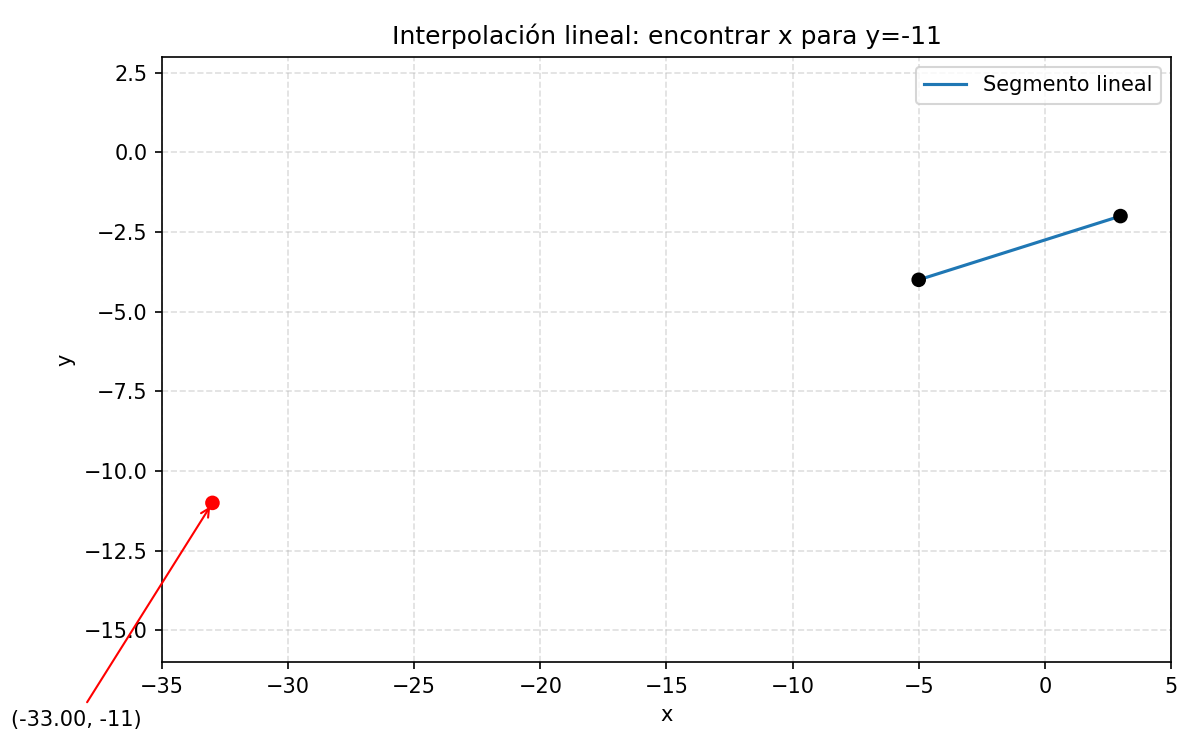
\includegraphics[width=0.75\textwidth]{linear_interp_yminus11.png}
    \caption{Captura de resultados de la interpolación lineal para $y=-11$.}
\end{figure}

\subsubsection*{b) Encontrar la ordenada en $x=-6$}
Los puntos son $(-3,2)$ y $(-4,-7)$.
La pendiente de la recta es:
\[
m = \frac{-7 - 2}{-4 - (-3)} = 9.
\]
La ecuación de la recta es:
\[
y - 2 = 9(x + 3).
\]
Para $x=-6$ se obtiene:
\[
y - 2 = 9(-6 + 3) = -27 \quad\Rightarrow\quad y = -25.
\]

\begin{figure}[H]
    \centering
    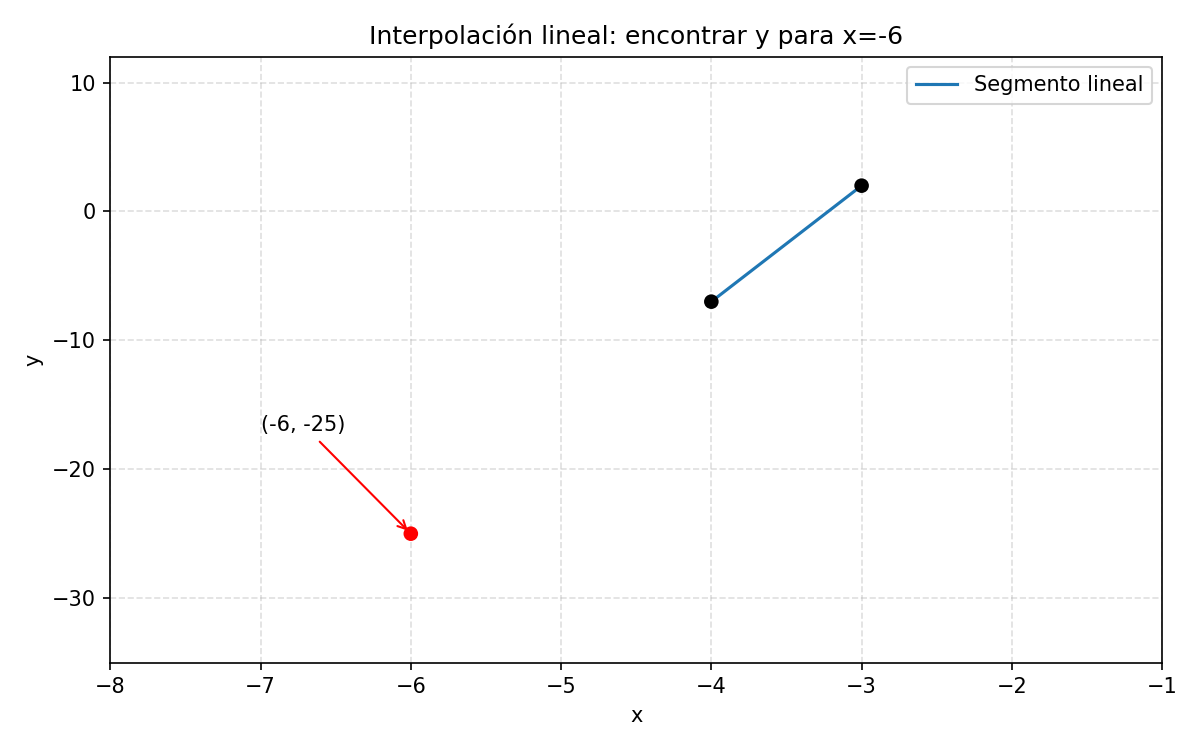
\includegraphics[width=0.75\textwidth]{linear_interp_xneg6.png}
    \caption{Captura de resultados de la interpolación lineal para $x=-6$.}
\end{figure}

\end{document}
